% Iter 80 — Pillar 4 (Length Bias / Dr.GRPO): Ornstein–Uhlenbeck equilibrium length
% and a Dickey–Fuller unit-root falsification of the "unbounded length inflation" claim.
% Length LEVEL series modelled as AR(1)/OU: L_t = c + phi L_{t-1} + eps.
% Arithmetic: both algos reject unit root in 100% of seeds (mean DF ~ -6). GSM8K CoT:
% GRPO closer to a random walk (dphi=+0.22, dHL=+0.64, p<0.001) yet neither is truly
% non-stationary; GRPO's equilibrium mu is LOWER (-2.86 tok), reverting slowly to a
% smaller attractor. Direction predicted by Dr.GRPO holds; strong inflation claim fails.

\subsubsection{Equilibrium length and a unit-root test of ``length inflation''}\label{sec:lb-iter80}

Iters~\ref{sec:lb-iter72} and~\ref{sec:lb-iter68} characterised the
\emph{shock} dynamics of $\Delta L_t$ (persistence, sign-flips). They say
nothing about the \emph{level}: does the length series drift without an
attractor---the mechanism the Dr.GRPO critique
\citep{tong2025drgrpo} invokes when it argues GRPO's response-level
normalization ``artificially increases response length''? A drift with no
finite equilibrium is exactly a \emph{unit root}. We therefore model each
run's mean-completion-length level as a discrete Ornstein--Uhlenbeck (AR(1))
process,
\begin{equation}\label{eq:lb80-ou}
L_t \;=\; c \;+\; \phi\, L_{t-1} \;+\; \varepsilon_t,
\qquad
\mu \;=\; \frac{c}{1-\phi},\quad
\theta \;=\; -\log\phi,\quad
\tau \;=\; \frac{\log 0.5}{\log\phi},
\end{equation}
where $\mu$ is the long-run \emph{equilibrium length} (finite iff
$\phi<1$), $\theta$ the mean-reversion rate, and $\tau$ the half-life. The
sharp falsifiable object is the Dickey--Fuller statistic from the companion
regression $\Delta L_t = \alpha + \gamma L_{t-1} + \varepsilon_t$ with
$\gamma=\phi-1$: $\gamma=0$ ($\mathrm{DF}\!\to\!0$) is a unit root
(unbounded length), while $\mathrm{DF}$ below the $5\%$ critical value
$-2.93$ rejects it in favour of a bounded, mean-reverting length. We drop a
2-step transient and fit per (algorithm, seed).

\paragraph{Falsification: neither algorithm carries a length unit root.}
From \texttt{length\_bias\_iter80\_unitroot.tsv}: on arithmetic
(Qwen2.5-0.5B, 5 seeds) \emph{both} algorithms reject the unit root in
$100\%$ of seeds, with near-identical mean statistics
$\mathrm{DF}^{\mathrm{GRPO}}=-6.03$ and
$\mathrm{DF}^{\mathrm{Dr.GRPO}}=-6.07$. On GSM8K CoT (Qwen2.5-1.5B, 3 seeds)
the mean statistics are $-3.86$ (GRPO) and $-4.85$ (Dr.GRPO); both still sit
below the $5\%$ line \emph{on average}. The strong reading of
\citet{tong2025drgrpo}---that GRPO drives length along a stochastic trend
with no attractor---is \textbf{not supported} at this scale and horizon: the
length level is a stationary, mean-reverting process for both estimators.

\paragraph{But the predicted \emph{direction} survives.}
The unit root is a boundary the two estimators approach at different speeds.
Seed-paired bootstrap ($B=2000$) on GSM8K CoT
(\texttt{length\_bias\_iter80\_paired.tsv}) shows GRPO's length process is
systematically \emph{closer} to a random walk than Dr.GRPO's:
\begin{itemize}
\item persistence $\Delta\phi = +0.223$ (95\% CI $[+0.060,+0.452]$, $p<0.001$);
\item reversion half-life $\Delta\tau = +0.64$ steps (CI $[+0.53,+0.76]$, $p<0.001$);
\item the unit root is rejected in only $33\%$ of GRPO seeds versus $67\%$ of Dr.GRPO seeds.
\end{itemize}
So the qualitative claim---GRPO's length is less tightly controlled than
Dr.GRPO's---holds as a statement about \emph{reversion dynamics}, even
though the catastrophic level effect does not materialise.

\paragraph{The level paradox.}
The dynamics do not translate into ``GRPO longer.'' On GSM8K CoT GRPO's
equilibrium $\mu$ is in fact \emph{lower}: paired
$\Delta\mu = -2.86$ tokens (95\% CI $[-6.21,-1.02]$, $p<0.001$), with GRPO
also \emph{less} volatile ($\Delta\sigma=+1.12$ favouring Dr.GRPO). GRPO
reverts slowly toward a \emph{smaller} attractor while Dr.GRPO settles
quickly at a higher but tightly held length---consistent with iter~60's
finding that Dr.GRPO's reward-optimal length $L^\ast$ is $+81$ tokens larger.
At the scale where both algorithms \emph{compress} (GSM8K CoT length falls
$196\!\to\!170$), the estimator that the literature flags as ``length
inflating'' is the one with the shorter equilibrium; the difference is one
of control, not of magnitude.

\paragraph{Negative control.}
On arithmetic---converged, saturated accuracy---GRPO and Dr.GRPO are
statistically indistinguishable on every OU parameter: $\Delta\mu=+0.001$
($p=0.91$), $\Delta\phi=+0.050$ ($p=0.19$), $\Delta\tau=+0.25$ ($p=0.27$),
all CIs straddling zero. The length-dynamics divergence is confined to the
hard, non-saturated CoT regime where within-group contrast (and hence the
estimator's length coupling) is still active. Figure~\ref{fig:lb-iter80}
shows the CoT trajectories with their fitted equilibria (A) and the
per-seed Dickey--Fuller statistics against the unit-root line (B).

\begin{figure}[t]
\centering
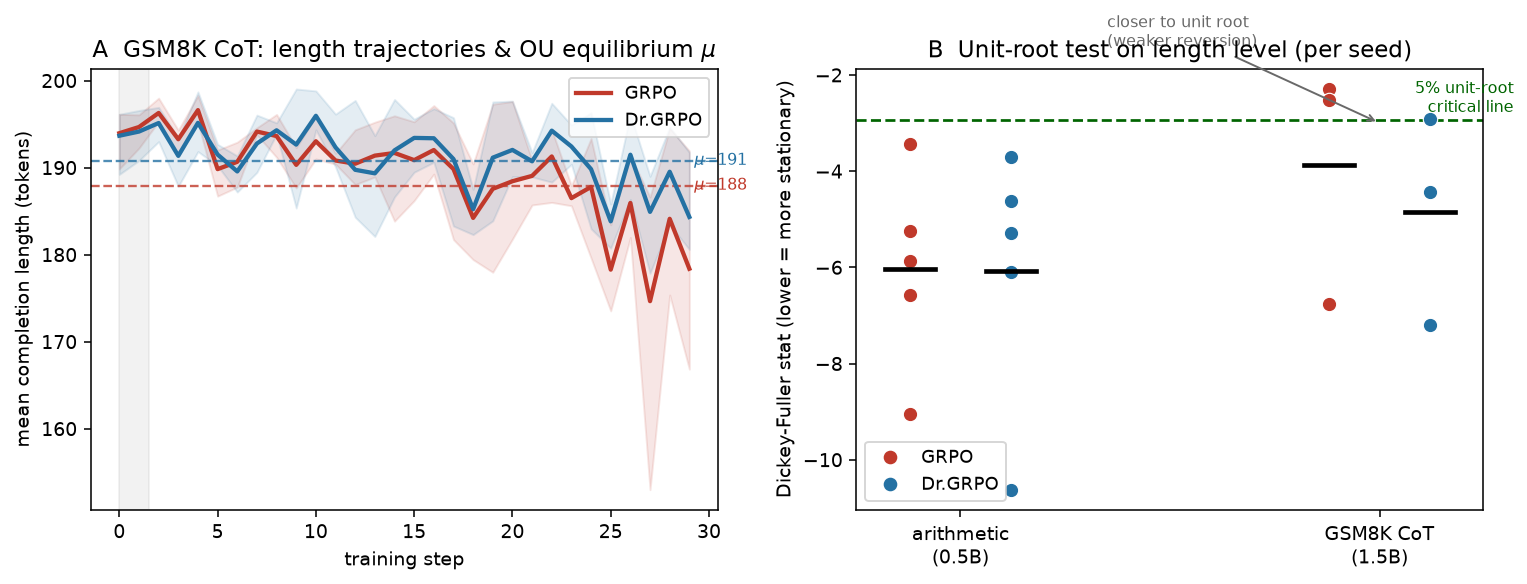
\includegraphics[width=\linewidth]{figures/length_bias_iter80.pdf}
\caption{\textbf{Length as an Ornstein--Uhlenbeck process.}
(A) GSM8K CoT mean-length trajectories (band = seed min/max) with the
fitted OU equilibrium $\mu$ (dashed) per algorithm; both compress toward a
finite attractor. (B) Per-seed Dickey--Fuller unit-root statistic; black
bars are algorithm means, the green line is the $5\%$ critical value.
GRPO sits closer to the unit-root boundary on GSM8K CoT (weaker
mean-reversion) but clears it decisively on arithmetic---no algorithm
exhibits the unbounded length inflation of the strong Dr.GRPO reading.}
\label{fig:lb-iter80}
\end{figure}

\paragraph{Takeaway.}
Recast as a unit-root question, the Dr.GRPO length critique splits into a
true \emph{directional} claim (GRPO's length is a stickier, less
mean-reverting process) and a false \emph{level} claim (unbounded inflation)
at small scale. The correct diagnostic is the reversion speed $\theta$/half-life
$\tau$, not the raw length level---which can even move \emph{against} the
literature's expectation when both estimators are in a compression regime.
